\section*{Blatt 23}

\newpage

\paragraph{Aufgabe 23.4(H)}

\begin{enumerate}

\item[]

Gegeben sei $y^2-4x=0$ und $x^2-4y=0$, dann gilt
\begin{align}
y^2-4x=0
\left\{
\begin{array}{lcl}
x=\frac{1}{4}y^2 \\
y=2\sqrt{x}
\end{array}
\right. \\
x^2-4y=0
\left\{
\begin{array}{lcl}
x=2\sqrt{y} \\
y=\frac{1}{4}x^2
\end{array}
\right.
\end{align}
dann die Schnittpunkten sind
\begin{align}
S_1(0,0) \\
S_2(4,4)
\end{align}
wie in der Abbildung gezeichnet
\begin{center}

\tikzset{every picture/.style={line width=0.75pt}} %set default line width to 0.75pt        

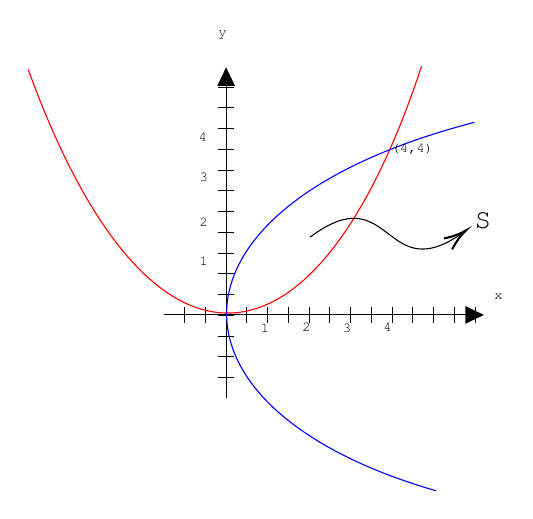
\begin{tikzpicture}[x=0.75pt,y=0.75pt,yscale=-1,xscale=1]
%uncomment if require: \path (0,266); %set diagram left start at 0, and has height of 266

%Shape: Boxed Line [id:dp5249456816593141] 
\draw    (5,223) -- (156.16,223) (15,219) -- (15,227)(25,219) -- (25,227)(35,219) -- (35,227)(45,219) -- (45,227)(55,219) -- (55,227)(65,219) -- (65,227)(75,219) -- (75,227)(85,219) -- (85,227)(95,219) -- (95,227)(105,219) -- (105,227)(115,219) -- (115,227)(125,219) -- (125,227)(135,219) -- (135,227)(145,219) -- (145,227)(155,219) -- (155,227) ;
\draw [shift={(159.16,223)}, rotate = 180] [fill={rgb, 255:red, 0; green, 0; blue, 0 }  ][line width=0.08]  [draw opacity=0] (8.93,-4.29) -- (0,0) -- (8.93,4.29) -- cycle    ;
%Straight Lines [id:da8945705280015244] 
\draw    (35,263.22) -- (35,106.72) (31,253.22) -- (39,253.22)(31,243.22) -- (39,243.22)(31,233.22) -- (39,233.22)(31,223.22) -- (39,223.22)(31,213.22) -- (39,213.22)(31,203.22) -- (39,203.22)(31,193.22) -- (39,193.22)(31,183.22) -- (39,183.22)(31,173.22) -- (39,173.22)(31,163.22) -- (39,163.22)(31,153.22) -- (39,153.22)(31,143.22) -- (39,143.22)(31,133.22) -- (39,133.22)(31,123.22) -- (39,123.22)(31,113.22) -- (39,113.22) ;
\draw [shift={(35,103.72)}, rotate = 90] [fill={rgb, 255:red, 0; green, 0; blue, 0 }  ][line width=0.08]  [draw opacity=0] (8.93,-4.29) -- (0,0) -- (8.93,4.29) -- cycle    ;
%Curve Lines [id:da9882251608059343] 
\draw [color={rgb, 255:red, 255; green, 0; blue, 0 }  ,draw opacity=1 ]   (-60.34,104.72) .. controls (-3.34,262.22) and (77.16,260.72) .. (129.16,103.22) ;
%Curve Lines [id:da586534056385196] 
\draw [color={rgb, 255:red, 0; green, 0; blue, 255 }  ,draw opacity=1 ]   (154.66,130.22) .. controls (-1.84,170.72) and (-0.84,268.22) .. (136.16,307.72) ;
%Curve Lines [id:da7084881277649522] 
\draw    (75.5,185.5) .. controls (115.1,155.8) and (110.75,211.09) .. (149.47,183.09) ;
\draw [shift={(150.66,182.22)}, rotate = 143.13] [color={rgb, 255:red, 0; green, 0; blue, 0 }  ][line width=0.75]    (10.93,-3.29) .. controls (6.95,-1.4) and (3.31,-0.3) .. (0,0) .. controls (3.31,0.3) and (6.95,1.4) .. (10.93,3.29)   ;

% Text Node
\draw (50.5,226) node [anchor=north west][inner sep=0.75pt]   [align=left] {{\fontfamily{pcr}\selectfont {\tiny 1}}};
% Text Node
\draw (70.5,225.5) node [anchor=north west][inner sep=0.75pt]   [align=left] {{\tiny {\fontfamily{pcr}\selectfont 2}}};
% Text Node
\draw (90,226) node [anchor=north west][inner sep=0.75pt]   [align=left] {{\fontfamily{pcr}\selectfont {\tiny 3}}};
% Text Node
\draw (109.5,225.5) node [anchor=north west][inner sep=0.75pt]   [align=left] {{\tiny {\fontfamily{pcr}\selectfont 4}}};
% Text Node
\draw (21,194) node [anchor=north west][inner sep=0.75pt]   [align=left] {{\fontfamily{pcr}\selectfont {\tiny 1}}};
% Text Node
\draw (21,175) node [anchor=north west][inner sep=0.75pt]   [align=left] {{\tiny {\fontfamily{pcr}\selectfont 2}}};
% Text Node
\draw (21,153.5) node [anchor=north west][inner sep=0.75pt]   [align=left] {{\fontfamily{pcr}\selectfont {\tiny 3}}};
% Text Node
\draw (20.5,134) node [anchor=north west][inner sep=0.75pt]   [align=left] {{\tiny {\fontfamily{pcr}\selectfont 4}}};
% Text Node
\draw (113.5,139.5) node [anchor=north west][inner sep=0.75pt]   [align=left] {{\fontfamily{pcr}\selectfont {\tiny (4,4)}}};
% Text Node
\draw (163,211.5) node [anchor=north west][inner sep=0.75pt]   [align=left] {{\fontfamily{pcr}\selectfont {\tiny x}}};
% Text Node
\draw (30,84.87) node [anchor=north west][inner sep=0.75pt]   [align=left] {{\fontfamily{pcr}\selectfont {\tiny y}}};
% Text Node
\draw (153.5,172.5) node [anchor=north west][inner sep=0.75pt]   [align=left] {{\fontfamily{pcr}\selectfont S}};

\end{tikzpicture}
\end{center}
Die Fläche ist gegeben als
\begin{align}
S
&=\int_0^4\int_{\frac{1}{4}x^2}^{2\sqrt{x}}dydx \\
&=\int_0^4 2\sqrt{x}dx-\int_0^4\frac{1}{4}x^2 dx \\
&=\bigg[
\frac{4}{3}x^{\sfrac{3}{2}}
\bigg]_0^4
-
\bigg[
\frac{1}{12}x^3
\bigg]_0^4 \\
&=\frac{16}{3}
\end{align}

\end{enumerate}

\newpage

\paragraph{Aufgabe 23.5(H)}

\begin{enumerate}

\item[]

Gegeben sei das Integral
\begin{align}
\int_{\frac{1}{2}}^{\frac{3}{2}}
\frac{x+\frac{1}{2}}{\sqrt{x^2-x+\frac{5}{4}}}dx
\end{align}
umformen
\begin{align}
=&\int_{\frac{1}{2}}^{\frac{3}{2}}\frac{x+\frac{1}{2}}{\sqrt{x^2-x+\frac{1}{4}+1}}dx \\
=&\int_{\frac{1}{2}}^{\frac{3}{2}}\frac{x+\frac{1}{2}}{\sqrt{(x-\frac{1}{2})^2+1}}dx 
\end{align}
Substitution $u=x-\frac{1}{2}$ mit $du=dx$, gilt
\begin{align}
\int_0^1\frac{u+1}{\sqrt{u^2+1}}du	
\end{align}
Substitution $u=\tan(v)$ mit $du=\sec^2(v)dv$
\begin{align}
&\int_0^{\frac{\pi}{4}}(\tan(v)+1)\frac{\sec^2(v)}{\sec(v)}dv \\
=&\int_0^{\frac{\pi}{4}}(\tan(v)+1)\sec(v)dv \\
=&\int_0^{\frac{\pi}{4}}(\tan(v)\sec(v)+\sec(v))dv \\
=&\int_0^{\frac{\pi}{4}}\tan(v)\sec(v)dv+\int_0^{\frac{\pi}{4}}\sec(v)dv \\
=&
\bigg[
\sec(v)
\bigg]_0^{\frac{\pi}{4}}
-
\bigg[
\ln|\tan(v)+\sec(v)|
\bigg]_0^{\frac{\pi}{4}} \\
=&\sqrt{2}-1+\ln(1+\sqrt{2})
\end{align}

\end{enumerate}